\begin{frame}[allowframebreaks]{Neural Autoregressive Density Estimation (NADE)}
\textbf{Introduced by:} Larochelle and Murray (2011)

\textbf{Goal:} Provide an efficient and scalable version of Fully Visible Sigmoid Belief Networks (FVSBN) by using shared weights and a feedforward neural network.

\textbf{Main Idea:}
\begin{itemize}
    \item Uses a masked neural network to estimate each conditional probability:
    \vspace{-0.5em}
    \begin{equation*}
        p(\mathbf{x}) = \prod_{i=1}^n p(x_i \mid x_{<i})
    \end{equation*}
    \vspace{-0.5em}
    \item Efficiently computes gradients via weight sharing and dynamic masking.
\end{itemize}

\textbf{Advantages:}
\begin{itemize}
    \item Tractable and scalable.
    \item Inspired later models such as MADE and normalizing flows.
\end{itemize}

\framebreak
\textbf{Model Structure:}
\begin{itemize}
    \item Each variable $x_i$ is modeled conditionally on all previous variables $x_{<i}$.
    \item Uses a neural network to compute the conditional probabilities.
    \item The weights are shared across different variables, reducing the number of parameters significantly.
\end{itemize}
\textbf{Formulation:}
\begin{itemize}
    \item The conditional probability is modeled as:
    \begin{equation*}
        p(x_i \mid x_{<i}) = \sigma(\alpha^{(i)} h_i + b_i)
    \end{equation*}
    where $h_i$ is a hidden representation computed from the previous variables, $\alpha^{(i)}$ are the weights, and $b_i$ is a bias term.
\end{itemize}
\textbf{Neural Network Layer:}

NADE uses a neural network layer instead of just logistic regression to improve model performance.
    $$h_i = \sigma(\mathbf{W}_{.,<i} x_{<i} + c)$$
    $$f_i(x_1,x_2,\cdots,x_{i-1}) = \sigma(\alpha^{(i)}h_i+b_i)$$

\framebreak

\begin{figure}
    \centering
    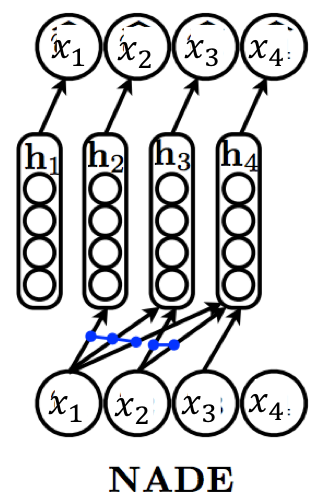
\includegraphics[height=0.7\textheight,keepaspectratio]{images/autoregressive/nade.png}
    \caption*{A neural autoregressive density estimator over four variables. Blue connections donate shared weights.}
\end{figure}

\end{frame}

\begin{frame}{NADE Results}

\begin{figure}
    \centering
    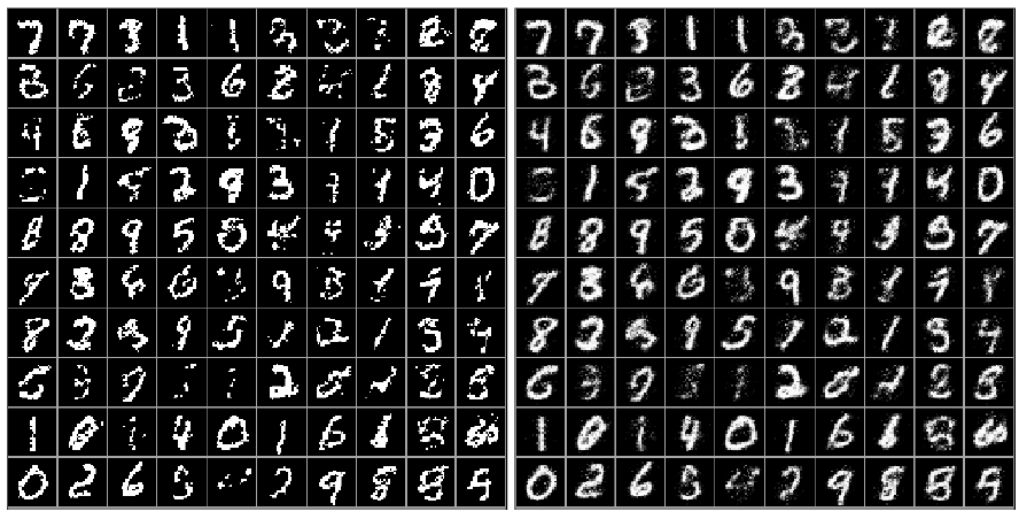
\includegraphics[height=0.7\textheight,keepaspectratio]{images/autoregressive/nade_results.png}
    \caption*{NADE results. Left: Samples generated by model. Right: Conditional Probabilities $\hat{x}_i$ (The Neural Autoregressive Distribution Estimator, 2011)}
\end{figure}

\end{frame}